% !TeX root = ..\studio-operation-guide.tex
\section{Call Transfer}
You can transfer a call to another party in one of three ways:

\begin{itemize}
	\item \textbf{Blind Transfer:} Transfer a call directly to another party
		without consulting.
	\item \textbf{Semi-Attended Transfer:} Transfer a call when the target phone
		is ringing.
	\item \textbf{Attended Transfer:} Transfer a call with prior consulting.
\end{itemize}

\subsubsection{To perform a blind transfer:}

\begin{enumerate}
	\item Press	\scalerel*{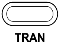
\includegraphics{images/yealink/btn-transfer.png}}{B}
		or the \textbf{Transfer} soft key during a call.
	\item Do one of the following:
	\begin{itemize}
		\item Enter the number you want to transfer the call to.
	\end{itemize}
	\item Press \scalerel*{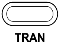
\includegraphics{images/yealink/btn-transfer.png}}{B}
		to complete the transfer.

		Then the call is connected to the number to which you are transferring.
\end{enumerate}

\subsubsection{To perform a semi-attended transfer:}

\begin{enumerate}
	\item Press	\scalerel*{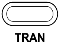
\includegraphics{images/yealink/btn-transfer.png}}{B}
		or the \textbf{Transfer} soft key during a call.
		\item Do one of the following:
		\begin{itemize}
			\item Enter the number you want to transfer the call to.
			\item Press the \textbf{Directory} soft key, and then select
				\textbf{Local Directory}. Select the desired group, and search
				for the contact (Directory should be configured in advance.
				Refer to Local Directory on page 33 for more information.).
			\item Press the \textbf{Directory} soft key, and then select History.
				Select the desired list and use
				\scalerel*{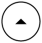
\includegraphics{images/yealink/btn-up.png}}{B} or
				\scalerel*{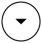
\includegraphics{images/yealink/btn-down.png}}{B} to
				select the entry (Directory should be configured in advance.
				Refer to Local Directory on page 33 for more information.).
			\item Press the \textbf{Directory} soft key, and then select 
				\textbf{Remote Phone Book}. Select the desired group and search
				for the contact (Directory and remote phone book should be
				configured in advance. Refer to Local Directory on page 33 and
				Remote Phone Book on page 46 for more information.)
	\end{itemize}
	\item Press \scalerel*{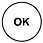
\includegraphics{images/yealink/btn-ok.png}}{B} or
		\scalerel*{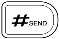
\includegraphics{images/yealink/btn-hash.png}}{B} to dial out.
	\item Press \scalerel*{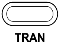
\includegraphics{images/yealink/btn-transfer.png}}{B}
		or the \textbf{Transfer} soft key to complete the transfer when
		receiving ringback.
\end{enumerate}

\subsubsection{To perform an attended transfer:}

\begin{enumerate}
	\item Press \scalerel*{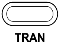
\includegraphics{images/yealink/btn-transfer.png}}{B}
		or the \textbf{Transfer} soft key during a call.
	\item Do one of the following:
	\begin{itemize}
		\item Enter the number you want to transfer the call to.
		\item Press the \textbf{Directory} soft key, and then select
			\textbf{Local Directory}. Select the desired group, and search for
			the contact (Directory should be configured in advance. Refer to
			Local Directory on page 33 for more information.).
		\item Press the \textbf{Directory} soft key, and then select
			\textbf{History}. Select the desired list and use
			\scalerel*{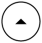
\includegraphics{images/yealink/btn-up.png}}{B} or
			\scalerel*{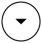
\includegraphics{images/yealink/btn-down.png}}{B} to
			select the entry (Directory should be configured in advance. Refer
			to Local Directory on page 33 for more information.).
			\item Press the \textbf{Directory} soft key, and then select 
				\textbf{Remote Phone Book}. Select the desired group and search
				for the contact (Directory and remote phone book should be
				configured in advance. Refer to Local Directory on page 33 and
				Remote Phone Book on page 46 for more information.)
		\end{itemize}
	\item Press the \textbf{Send} soft key,
		\scalerel*{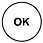
\includegraphics{images/yealink/btn-ok.png}}{B} or
		\scalerel*{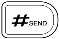
\includegraphics{images/yealink/btn-hash.png}}{B} to dial out.
	\item After the party answers the call, press
		\scalerel*{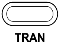
\includegraphics{images/yealink/btn-transfer.png}}{B} or the
		\textbf{Transfer} soft key to complete the transfer.
\end{enumerate}

If you are using a handset, the transfer can be completed by hanging up
the handset.

You can cancel the transfer before the call is connected by pressing the
\textbf{Cancel} soft key.